\documentclass{beamer}\usepackage[]{graphicx}\usepackage[]{color}
% maxwidth is the original width if it is less than linewidth
% otherwise use linewidth (to make sure the graphics do not exceed the margin)
\makeatletter
\def\maxwidth{ %
  \ifdim\Gin@nat@width>\linewidth
    \linewidth
  \else
    \Gin@nat@width
  \fi
}
\makeatother

\definecolor{fgcolor}{rgb}{0.345, 0.345, 0.345}
\newcommand{\hlnum}[1]{\textcolor[rgb]{0.686,0.059,0.569}{#1}}%
\newcommand{\hlstr}[1]{\textcolor[rgb]{0.192,0.494,0.8}{#1}}%
\newcommand{\hlcom}[1]{\textcolor[rgb]{0.678,0.584,0.686}{\textit{#1}}}%
\newcommand{\hlopt}[1]{\textcolor[rgb]{0,0,0}{#1}}%
\newcommand{\hlstd}[1]{\textcolor[rgb]{0.345,0.345,0.345}{#1}}%
\newcommand{\hlkwa}[1]{\textcolor[rgb]{0.161,0.373,0.58}{\textbf{#1}}}%
\newcommand{\hlkwb}[1]{\textcolor[rgb]{0.69,0.353,0.396}{#1}}%
\newcommand{\hlkwc}[1]{\textcolor[rgb]{0.333,0.667,0.333}{#1}}%
\newcommand{\hlkwd}[1]{\textcolor[rgb]{0.737,0.353,0.396}{\textbf{#1}}}%
\let\hlipl\hlkwb

\usepackage{framed}
\makeatletter
\newenvironment{kframe}{%
 \def\at@end@of@kframe{}%
 \ifinner\ifhmode%
  \def\at@end@of@kframe{\end{minipage}}%
  \begin{minipage}{\columnwidth}%
 \fi\fi%
 \def\FrameCommand##1{\hskip\@totalleftmargin \hskip-\fboxsep
 \colorbox{shadecolor}{##1}\hskip-\fboxsep
     % There is no \\@totalrightmargin, so:
     \hskip-\linewidth \hskip-\@totalleftmargin \hskip\columnwidth}%
 \MakeFramed {\advance\hsize-\width
   \@totalleftmargin\z@ \linewidth\hsize
   \@setminipage}}%
 {\par\unskip\endMakeFramed%
 \at@end@of@kframe}
\makeatother

\definecolor{shadecolor}{rgb}{.97, .97, .97}
\definecolor{messagecolor}{rgb}{0, 0, 0}
\definecolor{warningcolor}{rgb}{1, 0, 1}
\definecolor{errorcolor}{rgb}{1, 0, 0}
\newenvironment{knitrout}{}{} % an empty environment to be redefined in TeX

\usepackage{alltt}
\title{The Accuracy and Predictiveness of State-Level Presidential Polls}
\author{Brittany Alexander}
\usepackage{hyperref}
\usecolortheme{beaver}
\IfFileExists{upquote.sty}{\usepackage{upquote}}{}
\begin{document}

\begin{frame}
\titlepage
\end{frame}
\begin{frame}
\frametitle{Outline}
  \tableofcontents
\end{frame}





\section{Introduction to Presidential Election Polling}
\begin{frame}{Introduction to Presidential Election Polling}
\begin{itemize}
\item Presidential Election polls aim to predict both the winner and the proportion of votes for candidates nationwide and in individual states
\item Predicting the winners of states is important because a candidate must win the most electors which is largely determined who wins a state
\item The number of electors per states is the number of respresentives in Congress plus two.
\item We define a state as competitive if it's margin on election day is between -5 and 5 points. Competitive states are of more interest.
\end{itemize}
\end{frame}


\begin{frame}{Challenges of Using Polls to Predict Elections}
\begin{itemize}
\item Election polls are taken before the election and voters change their minds
\item Polls typically include undecided voters
\item It is common for polls to ignore minor candidates

\end{itemize}
\end{frame}

\begin{frame}{Data Source}
\href{https://elections.huffingtonpost.com/pollster}{Huffington Post Pollster} has polling data for 2012-2016.  There was a site to get 2008 data before Pollster merged with Huffington Post, but that link is broken. There are 5756 state level polls across the three elections. Most states have multiple polls for each election year. This data set also contains new variables to model polling across years. New variables includes:
\begin{itemize}
\item The election results as both the margin and the two party vote
\item Days until the election at the start, end, and middle of a poll
\item Various versions of polling error
\end{itemize}

\end{frame}


\section{Previous Work}
\begin{frame}{Inspiration}
\href{https://twitter.com/aedwardslevy/status/1138832357224525829}{Twitter Thread}
\begin{figure}[h]
       \centering
        \includegraphics[height = 0.75\textheight]{"twitterinspiration".png}
    \end{figure}
\end{frame}

\begin{frame}{Literature Review}
\begin{itemize}
\item Hillygus, D. S. (2011) describes a history of election polling but doesn't include much on state level polls
\item Bon et.al 2019 focused on the effects of undecided voters and polling bias
\item Shirani-Mehr (2018) built a model to decompose bias and variance in polls but focused on the last two weeks of the election
\item Alexander (2019) built a model and looks at the accuracy of averaging the polls
\item None of these studies focuses on individual polls during a broad range of time
\end{itemize}
\end{frame}

\section{Definition of Accuracy and Predictiveness}
\begin{frame}{Accuracy}
Accuracy in polling has two components: percent called correctly, and distance between a polls results and what happens on election day.  Additionally accuracy can be viewed in terms of margin, and in terms of vote. Margin is defined as the difference between the Democratic vote (or poll support) and the Republician vote (or poll support). Accuracy in terms of vote is measured by first applying the formula: $d_{new} = \frac{d}{d+r}, r_{new} = \frac{r}{d+r}$ to polls and vote results so that the Republican and Democratic support sums to 1. This standardizes results to deal with different levels of undecideds, and the inclusion of minor candidates.
\end{frame}

\begin{frame}{Predictiveness}
Predictiveness is defined by the strength of a correlation between two variables and $R^2$ of fit regressions. Predictiveness is matters because it tells us if and when we can consider polls to have predictive value in the election.  
\end{frame}

\section{The State of State Level Polls}
\begin{frame}{Accuracy Over Time}
One key question is how accurate polls are far out from election day. 200 days would be approximately in late January (start of the primary), and 100 days before is the end of August. This uses lowess smoothing. 

\begin{knitrout}
\definecolor{shadecolor}{rgb}{0.969, 0.969, 0.969}\color{fgcolor}
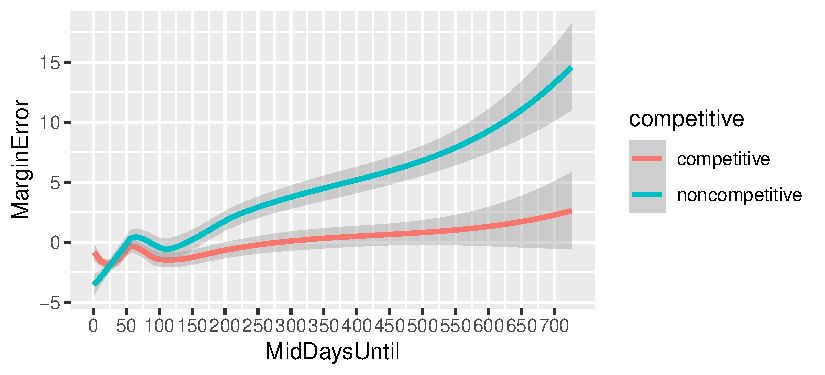
\includegraphics[width=\maxwidth]{figure/unnamed-chunk-2-1} 

\end{knitrout}
\end{frame}

\begin{frame}{Average Error By State}
Below is a Choropleth of the Average Polling Error in the last 60 days until the election.
%code is in plotlycode.R
\begin{figure}[h]
       \centering
        \includegraphics[width = 0.75\textwidth]{"AverageMarginPollingError08-16".png}
\end{figure}
\end{frame}

\begin{frame}{Accuracy By Partisanship}
Below is a plot of the Average Margin Error of polls from the last 60 days for a state by it's actual margin on election day. 
\begin{itemize}
\item Recall that proportions are most variable when they are closest to .5 suggesting that competitive states should have more sampling error.
\item Possible explaination: Nonsampling factors such as poll quality, frequency polled, etc.  explain this phenomon.
\end{itemize}
\begin{knitrout}
\definecolor{shadecolor}{rgb}{0.969, 0.969, 0.969}\color{fgcolor}
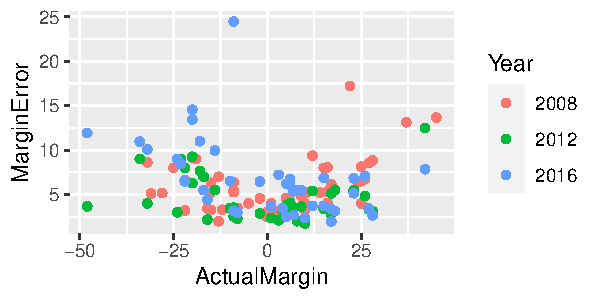
\includegraphics[width=\maxwidth]{figure/unnamed-chunk-3-1} 

\end{knitrout}

\end{frame}

\begin{frame}{Margin Error in Competitive and Non-Competitive States}
Below is a plot showing the average Margin error in competitive and noncompetitive states, broken up by week for the last 12 weeks of the election. Purple Square is competitive states, and Black Rhomus is noncompetitive states.
\begin{knitrout}
\definecolor{shadecolor}{rgb}{0.969, 0.969, 0.969}\color{fgcolor}
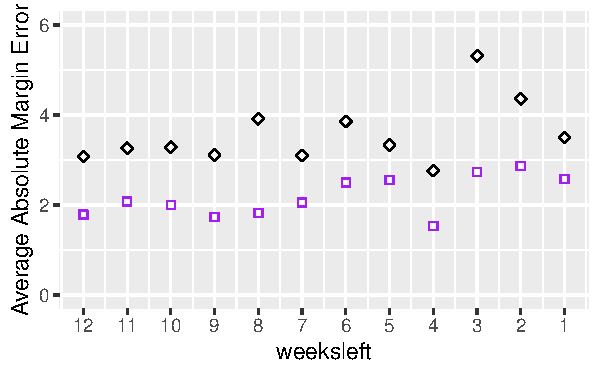
\includegraphics[width=\maxwidth]{figure/unnamed-chunk-4-1} 

\end{knitrout}

\end{frame}
\begin{frame}{Percent of Races Called Correctly}
Below is a plot of the percent of races called correctly. Purple Square is competitive states, and Black Rhomus is noncompetitive states.
\begin{knitrout}
\definecolor{shadecolor}{rgb}{0.969, 0.969, 0.969}\color{fgcolor}
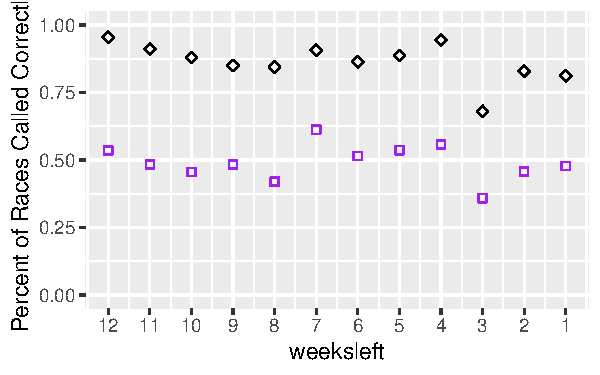
\includegraphics[width=\maxwidth]{figure/unnamed-chunk-5-1} 

\end{knitrout}
\end{frame}

\begin{frame}{Predictiveness Attempt 1}
\begin{itemize}
\item Below are estimated $R^2$ to predict the margin on election day given the polling margin for competitive and noncompetitive states. Purple Square is competitive states, and Black Rhomus is noncompetitive states.
\end{itemize}
\begin{knitrout}
\definecolor{shadecolor}{rgb}{0.969, 0.969, 0.969}\color{fgcolor}
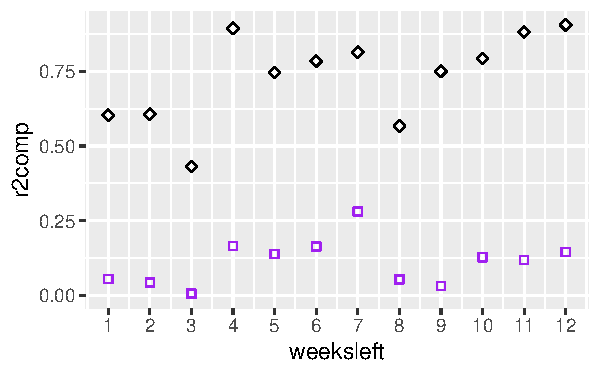
\includegraphics[width=\maxwidth]{figure/unnamed-chunk-6-1} 

\end{knitrout}

\end{frame}

\begin{frame}{Predictiveness Attempt 2}
\begin{itemize}
\item A mixed model including random effects for Year, State, and Year interacted with state is now fit.  We plot the psuedo $R^2$ for the mixed model. Purple Square is competitive states, and Black Rhomus is noncompetitive states.
\end{itemize}
\begin{knitrout}
\definecolor{shadecolor}{rgb}{0.969, 0.969, 0.969}\color{fgcolor}
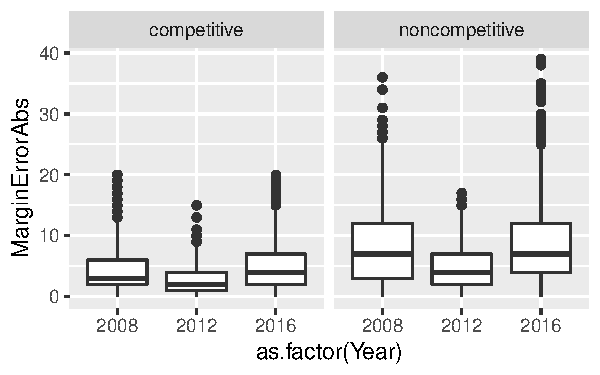
\includegraphics[width=\maxwidth]{figure/unnamed-chunk-7-1} 

\end{knitrout}

\end{frame}

\section{2016 Mythbusting}
\begin{frame}{2016 Errors were Not Abnormally Large}
\begin{itemize}
\item Polling Errors in 2008 were highly similar in absolute value to 2008. 2008 and 2012 broadly underestimated Democratic support, but in 2016 Republican support was underestimated.
\end{itemize}
\begin{knitrout}
\definecolor{shadecolor}{rgb}{0.969, 0.969, 0.969}\color{fgcolor}
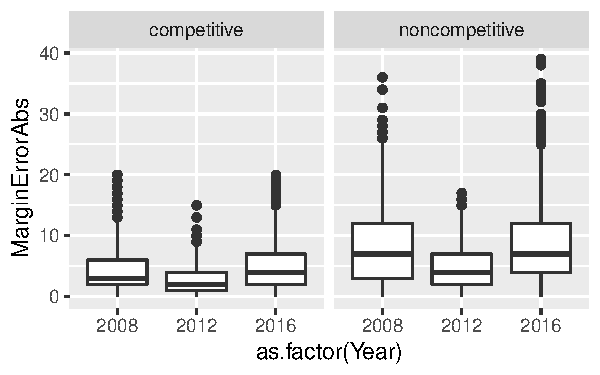
\includegraphics[width=\maxwidth]{figure/unnamed-chunk-8-1} 

\end{knitrout}
\end{frame}
\begin{frame}{Polling Errors in FL, MI, NC, PA, WI}
\begin{itemize}
\item Polling errors were not abnormally larger in 2016 in FL, MI, NC, PA, WI in terms of error, but the races were not called correctly.  
\end{itemize}
\begin{knitrout}
\definecolor{shadecolor}{rgb}{0.969, 0.969, 0.969}\color{fgcolor}
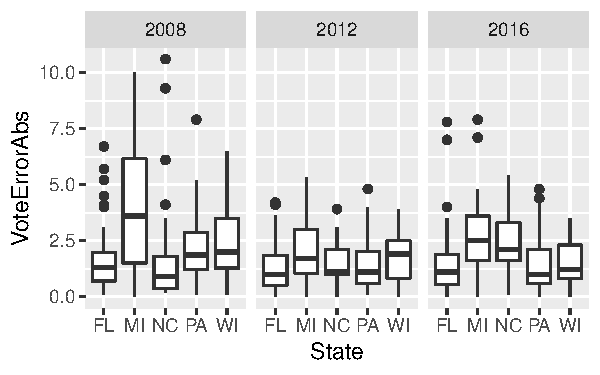
\includegraphics[width=\maxwidth]{figure/unnamed-chunk-9-1} 

\end{knitrout}
\end{frame}



\begin{frame}{Polling Errors in FL, MI, NC, PA, WI Part Two}
Below is a plot of polling errors in 2016, and we see that FL, MI, NC, PA, WI are not unsual compared to other states. %code is in plotlycode.R
\begin{figure}[h]
       \centering
        \includegraphics[width = 0.75\textwidth]{"AverageMarginPollingError2016".png}
    \end{figure}
\end{frame}


\section{Looking Forward to 2020}
\begin{frame}{Conclusion}
Polls have small predictive value throughout the election process due to inconsistent patterns across states and years. Polling Accuracy is relatively stable starting three weeks out.  A more controlled in depth analysis and model is needed to adjust for the differences in states, polling quality, and polling volume. However, it is clear that while polling error was larger in 2016 than 2012, it is similar to 2008.  The focus on FL, MI, NC, PA, WI being wrong ignores that the direction of sampling error is random and can not be controlled. Overall polls were reliable in those states compared to previous years.
\end{frame}

\begin{frame}{References}
\begin{itemize}
\item Alexander, Brittany (2019), "A Bayesian Model for the Prediction of United States Presidential Elections," \texit{SIAM Undergraduate Research Online}, \textbf{12}. 
\item Bon, J. J., Ballard, T., \& Baffour, B. (2019), "Polling bias and undecided voter allocations: US presidential elections, 2004–2016," \texit{Journal of the Royal Statistical Society: Series A (Statistics in Society)}, \textbf{182(2)}, 467-493.
\item Hillygus, D. S. (2011). "The evolution of election polling in the United States," \textit{Public opinion quarterly}, \textbf{75(5)}, 962-981
\item Shirani-Mehr, H., Rothschild, D., Goel, S., \& Gelman, A. (2018), "Disentangling bias and variance in election polls," \texti{Journal of the American Statistical Association}, \textbf{113(522)}, 607-614.
\end{itemize}
\end{frame}

\end{document}
